\documentclass[twocolumn]{article}

\usepackage[utf8]{inputenc}
\usepackage[english]{babel}
\usepackage{graphicx}
\usepackage{subcaption}
\usepackage{amsmath}
\usepackage{bbm}%per il simbolo del gradino
\usepackage{url}

\title{InSaNeQKD}
\author{}
\date{}

\begin{document}
	
	\maketitle
	
	\section{Introduction}
	[...]
	\section{Background noise estimation}
	In this section we analyze the background noise received by Bob in terms of average number of photons  sent by the environment, $N_{back}$: in particular, it's possible to estimate $N_{back}$ by using the simple equation
	\begin{equation}
	N_{back}= L(\lambda)\ \Omega\ \pi R_{aperture}^2\ t_d\ \Delta\lambda
	\end{equation}
	where $L(\lambda)$ is the noise radiance, measured in ${[\rm ph\ s^{-1}\ m^{-2}\ nm^{-1}]}$, $\Omega$ is the receiver field-of-view, measured in steradians, $R_{aperture}$ is the receiver's telescope radius, $t_d$ is the detection time and $\Delta\lambda$ is the bandwidth of the receiver filter. Notice that in our simulation we took $R_{\rm aperture}=15\ {\rm cm}$, $\Omega = 100\ {\rm \mu rad}$, $t_{\rm d} = 500\ {\rm ps}$ and $\Delta\lambda = 1\ {\rm nm}$.
	
	Hence taking different radiances $L(\lambda)$, we can estimate the noise $N_{back}$ for each of them: for example, as done in \cite{tomaello11}, we can consider the so-called sky brightness that models the contributions of multiple sources, like airglow, zodiacal light, integrated starlight and extragalactic background light: luckily, since in our model we are considering the intersatellite links between satellites in the MEO orbit, we can neglect the airglow that is the strongest noise source between the considered ones \cite{leinert98} since for the visible and infrared bandwidth, it is present on altitudes of around 80-100 km. Hence we can take $L( 800\ {\rm nm}) \simeq0.7\ [\rm nW\ m^{-2}\ nm^{-1}]\simeq2.8\ 10^{-9} {[\rm ph\ s^{-1}\ m^{-2}\ nm^{-1}]}$, obtaining $N_{back,sky}\simeq 3.1\ 10^{-9}$ photons.
	Other sources that may be considered are the sunlight and the moonlight: however, since the receiver $\Omega$ is usually narrow, the probability that the Sun (or the Moon) falls in the receiver field-of-view is essentially the probability that the Sun (or the Moon), transmitter and receiver are all aligned, so it's reasonably neglectable.
	
	A source that has never been analyzed or modeled in literature is the diffused sunlight, the light that reaches the receiver after being scattered by Alice or, in other terms, the noise that Bob obtains since he is watching an object illuminated by the Sun, Alice itself.
	Since we don't have the satellite's \textit{bidirectional reflectance distribution function} (BRDF), to analyze this effect we need to model the satellite shapes: in particular we consider two different simple shapes, a sphere of radius $R_{sat}= 1\ {\rm m}$ and a parallelepiped of dimensions ${\rm 2.7\ m\times\ 1.2\ m\times 1.1\ m}$, both covered by a Lambertian aluminum surface with albedo $a = 0.85$. 
	
	\subsection{Light scattered by the sphere}
	To model the scattered light radiance we divide the transmitter surface in k infinitesimal surfaces $dS$, hence using the Lambert's cosine law, each $dS$ gives a contribution of 
	\[
	L(\lambda,\theta_k) = \frac{a}{\pi}H_{\rm Sun}(\lambda) \cos(\theta_k)dS
	\]
	where $H_{Sun}$ is the \textit{Solar spectral irradiance} (SSI) and $\theta_k$ is the angle between the Sun and the $dS$ normal $\vec{n}$. Notice that to estimate the Solar spectral irradiance we used the SOURCE dataset \cite{SOURCEdataset}.
	Therefore the total radiance is simply
	\begin{equation}\label{eq:generalEq}
	L(\lambda) = \int_{S_{\rm sat}\bigcap S_{\rm Sun}} \frac{a}{\pi}H_{\rm Sun}(\lambda) \cos(\theta_k)dS
	\end{equation}
	where $S_{\rm sat}\bigcap S_{\rm Sun}$ is the intersection between the spherical cap seen by the receiver and the spherical cap that illuminated by the Sun; notice that since $R_{sat}\ll {\rm d(Sun,Alice),\ d(Alice,Bob)}$ both the spherical caps are approximately hemispheres.
	
	\begin{figure}[t]
		\centering
		\begin{subfigure}[b]{\linewidth}
			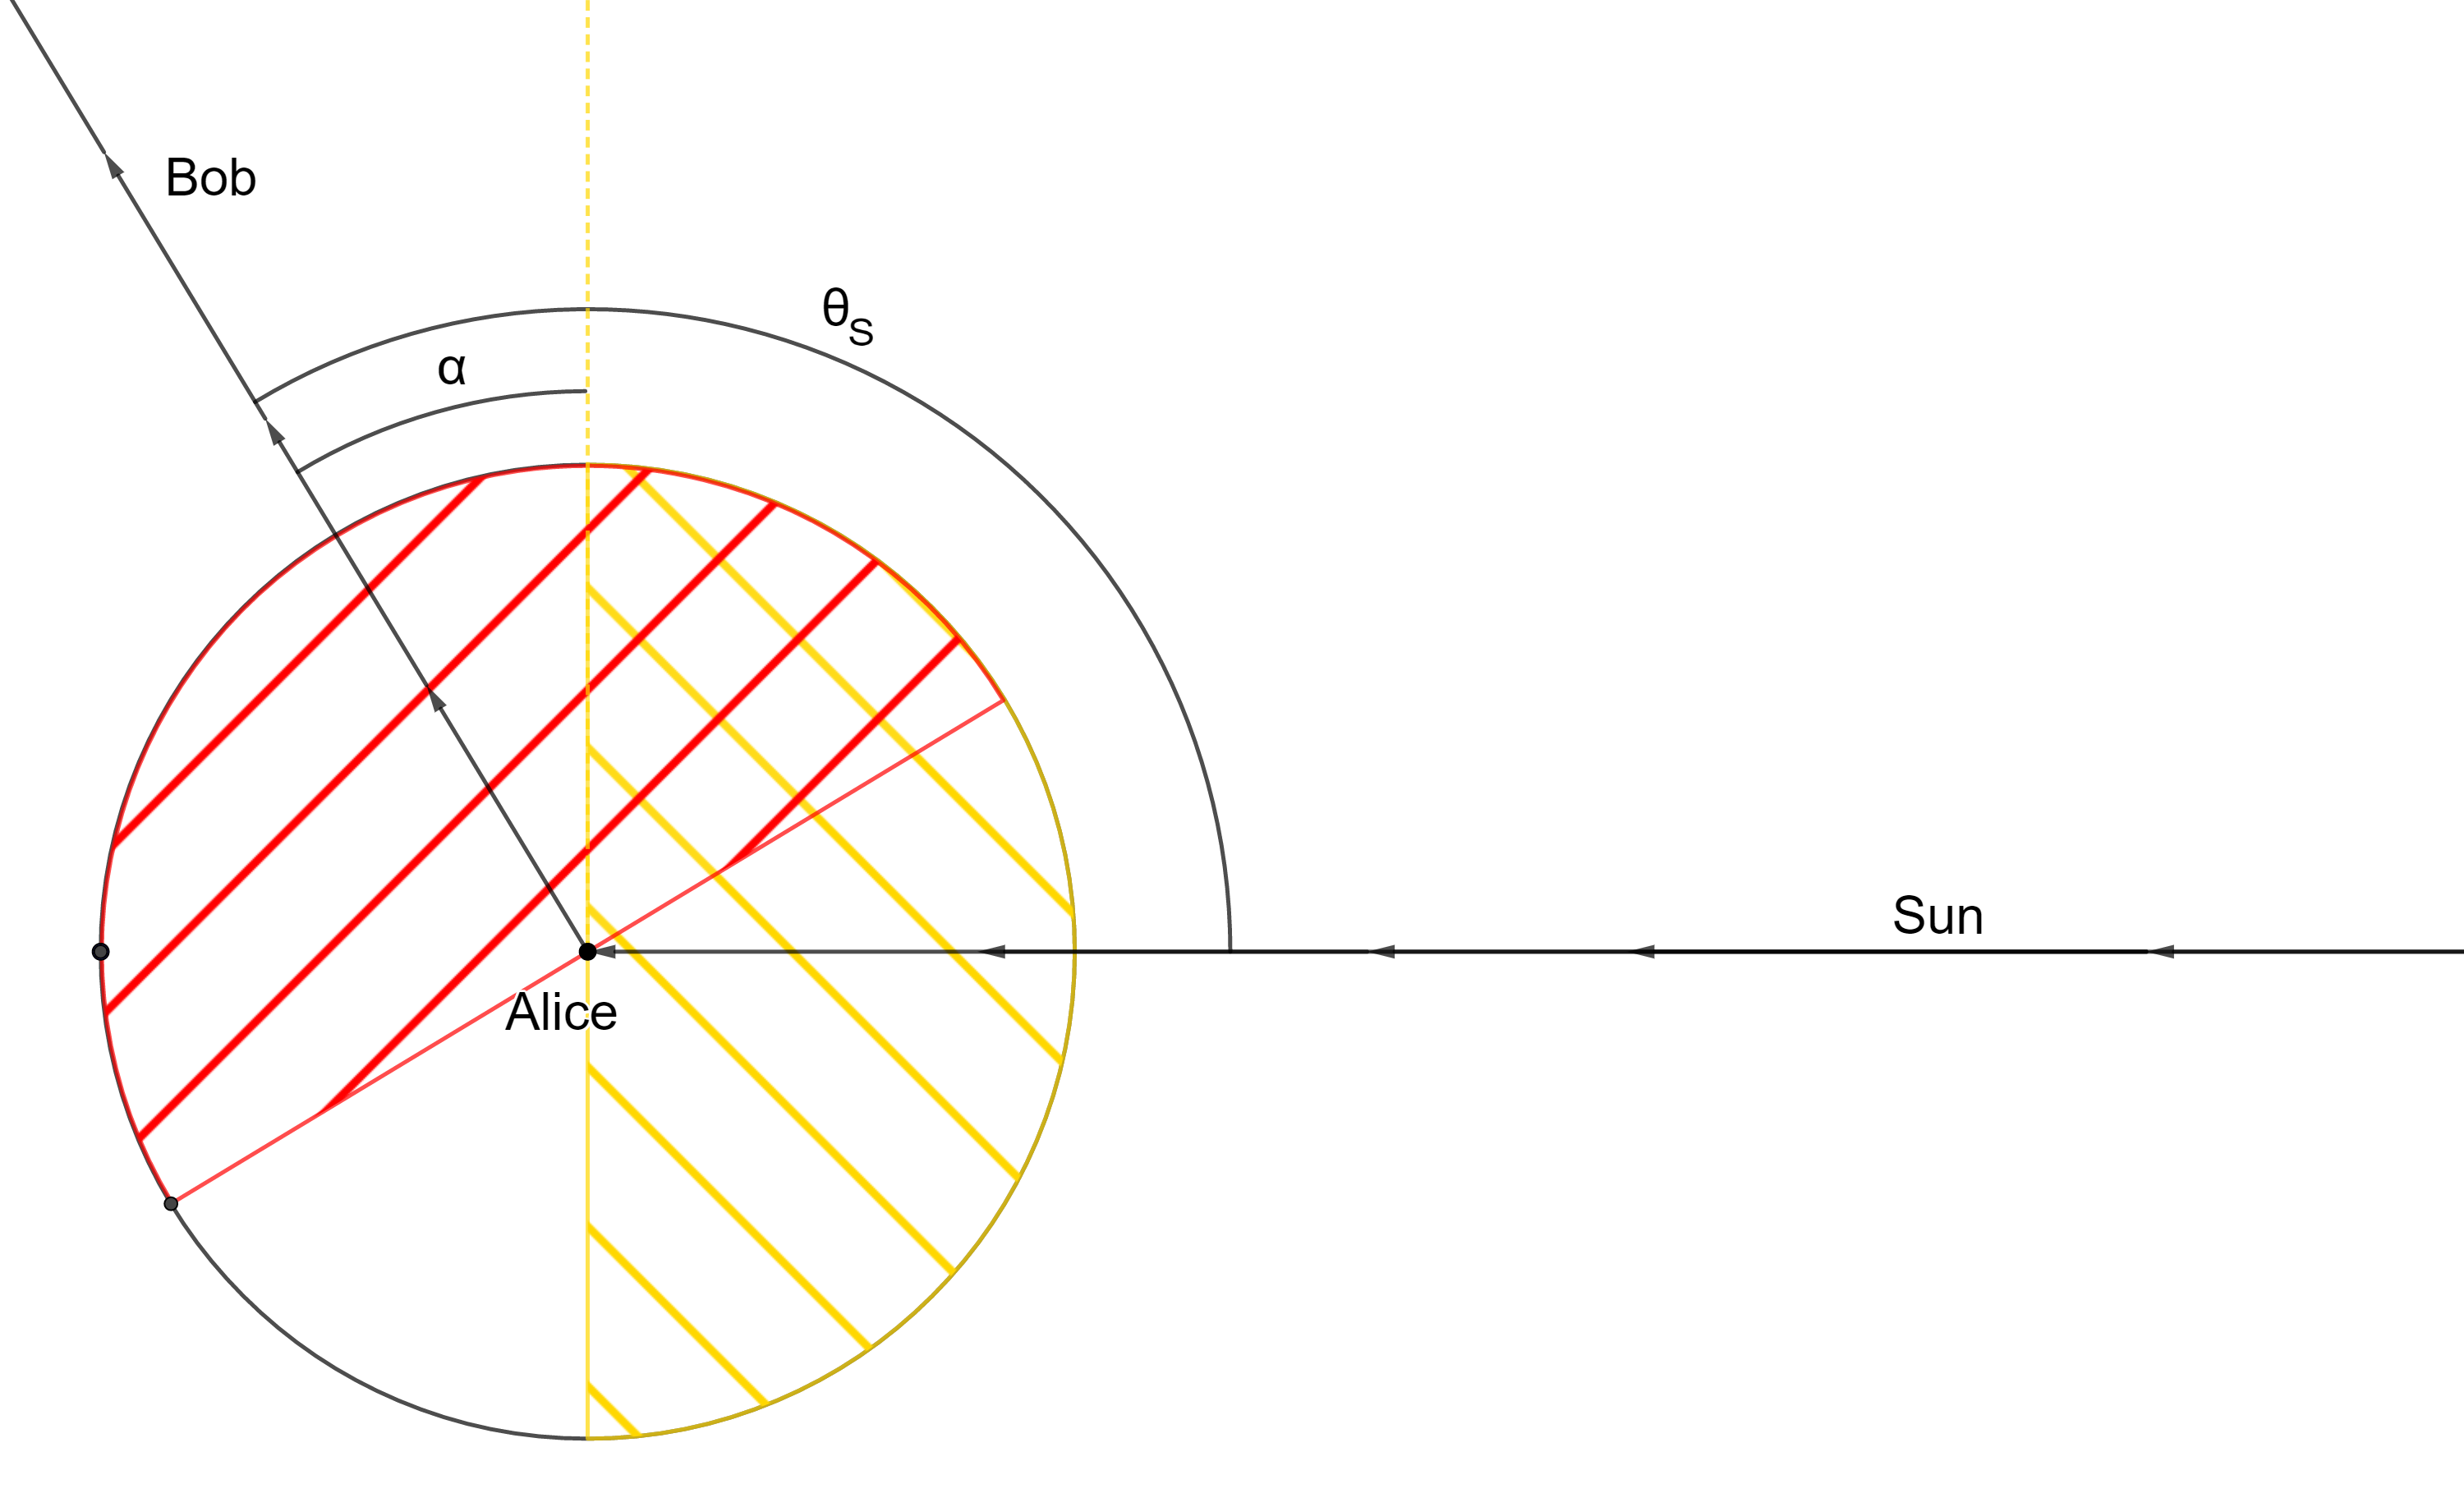
\includegraphics[width=\linewidth]{schema1.png}
			\caption{$\theta_S\geq \pi/2$}
			\label{fig:schema1}
		\end{subfigure}
		\begin{subfigure}[b]{\linewidth}
			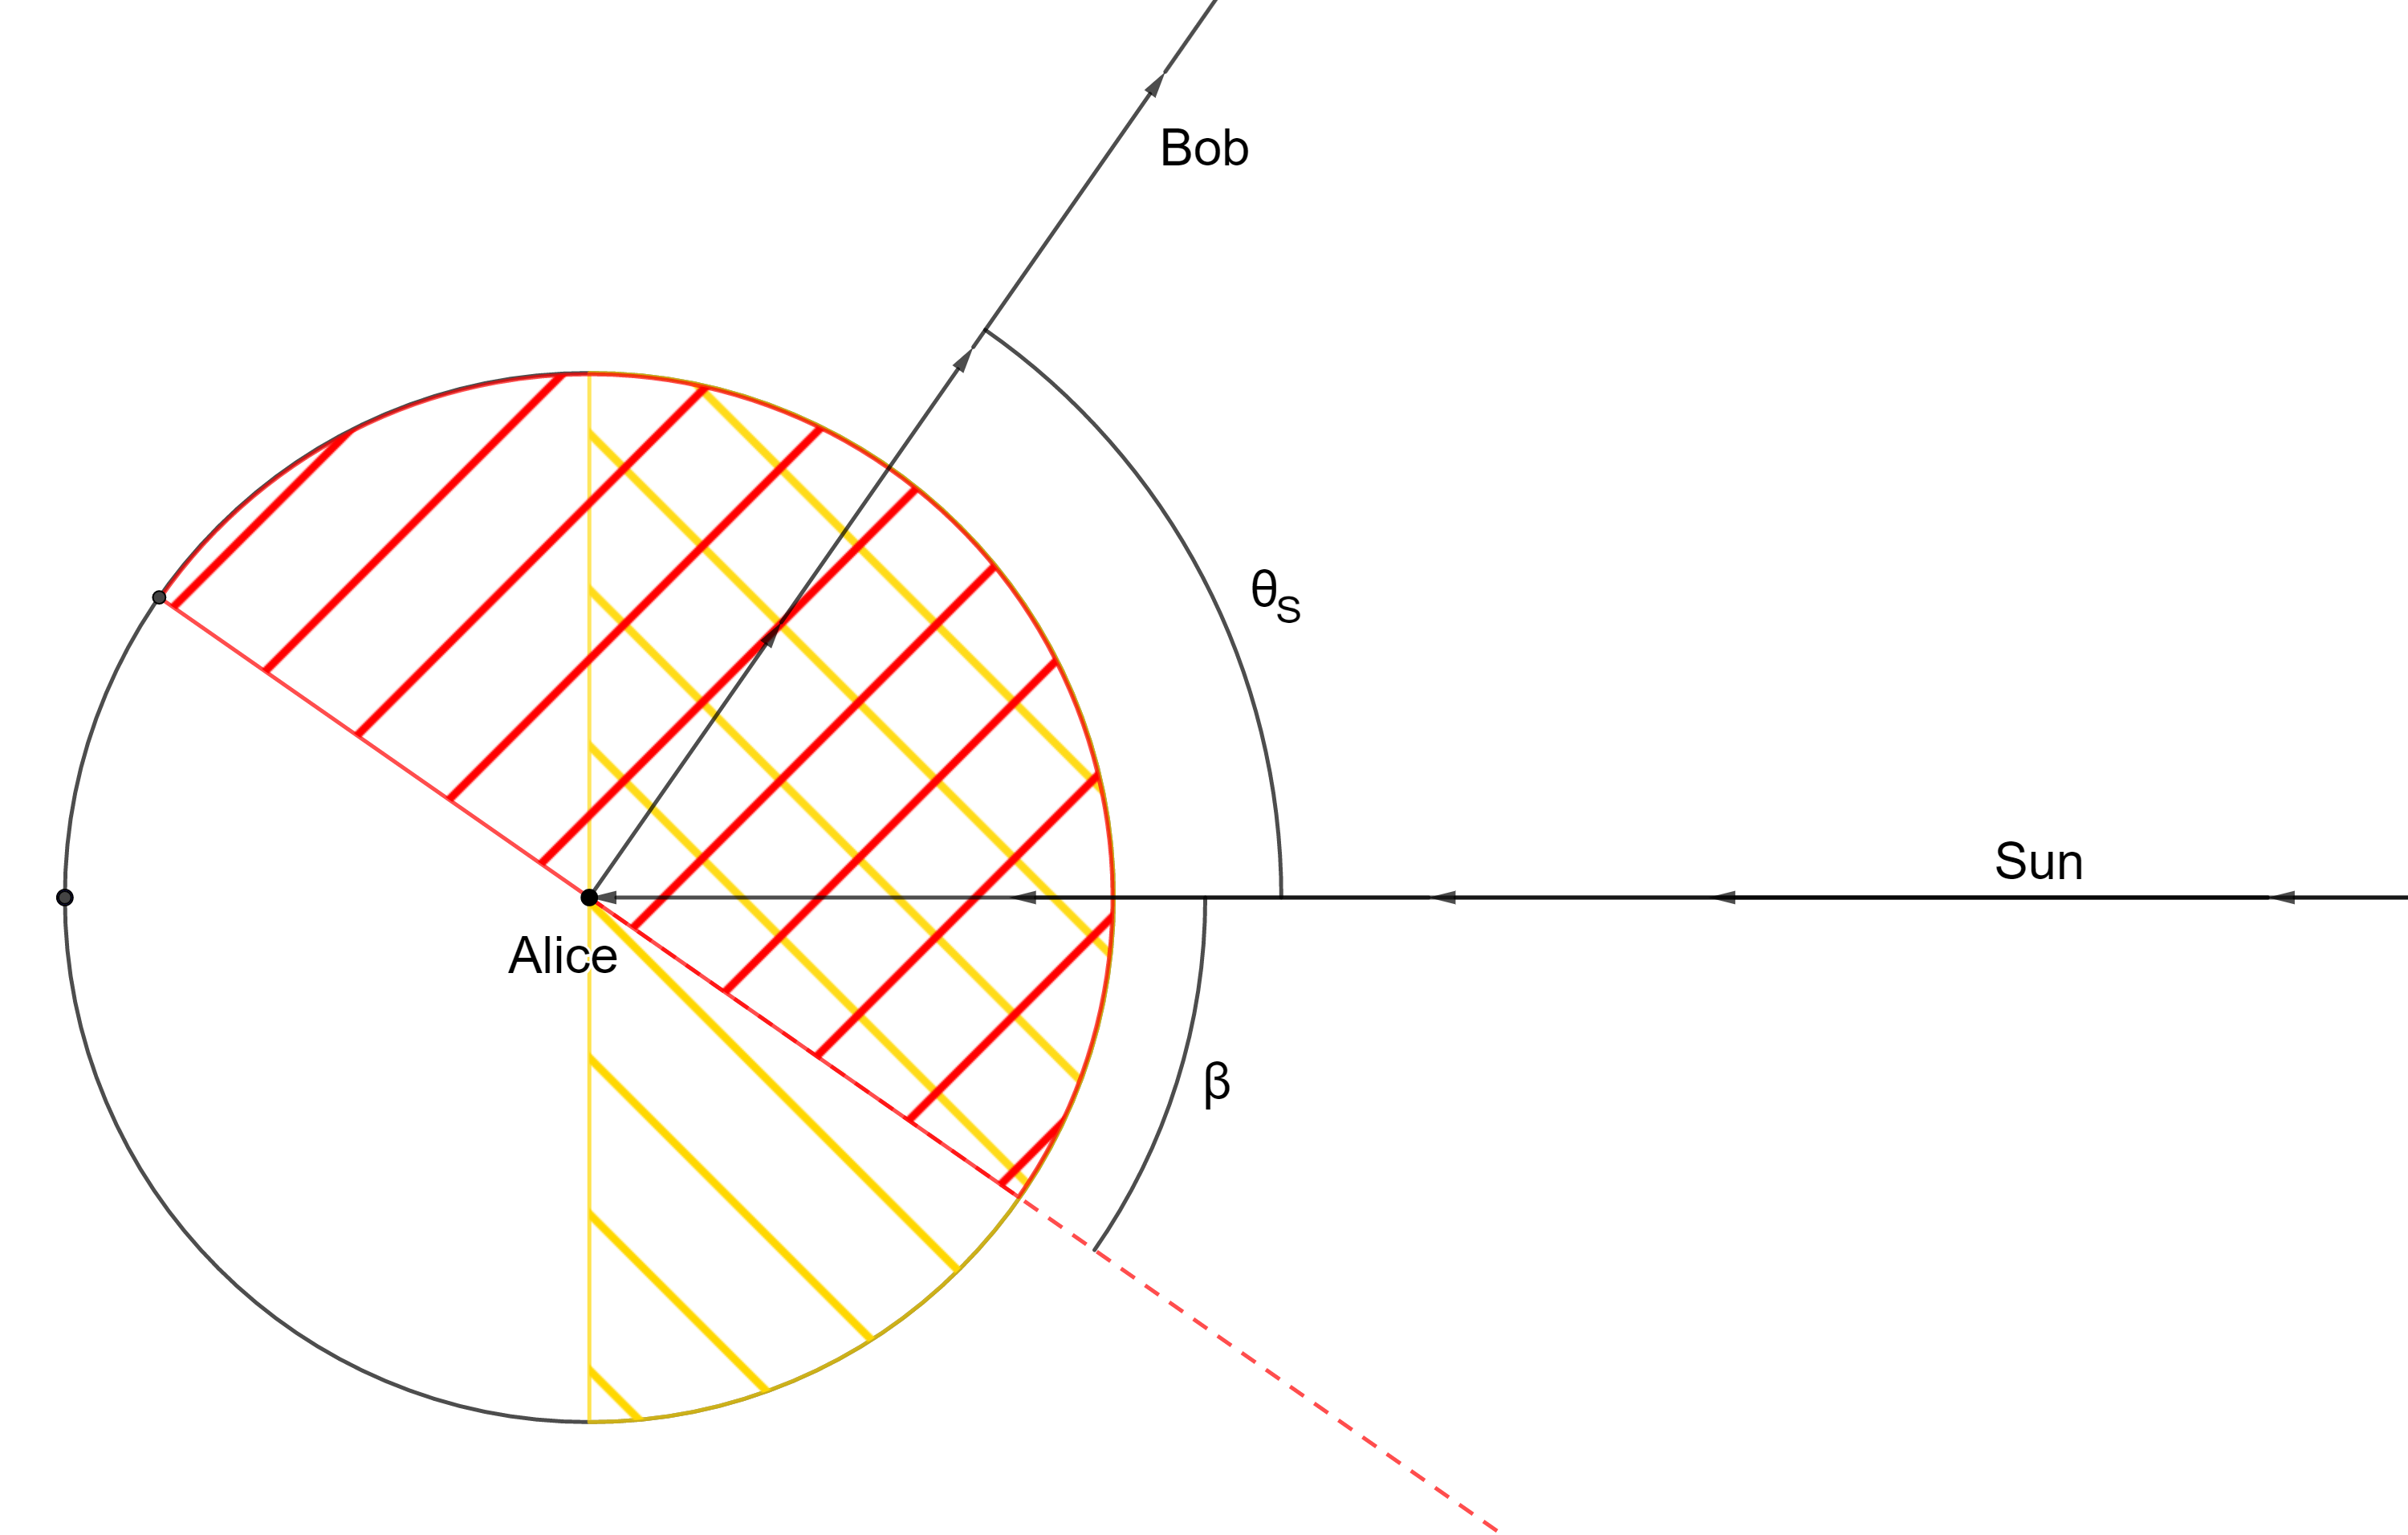
\includegraphics[width=\linewidth]{schema2.png}
			\caption{$\theta_S < \pi/2$}
			\label{fig:schema2}
		\end{subfigure}
		\caption{Schemes used for the estimation of the radiance $L_{\rm sphere}(\lambda,\theta_S)$, for the spherical model.}\label{fig:schemisfera}
	\end{figure}
	
	In order to compute this surface we consider the two cases pictured in Fig. \ref{fig:schemisfera}, where $\theta_S$ is the angle between the Sun, Alice and Bob, which can be easily computed as 
	\begin{equation}
	{\rm \theta_S = acos\bigg( \frac{d(Tx,Rx)^2+d(Tx,Sun)^2-d(Rx,Sun)^2}{2d(Tx,Rx)\ d(Tx,Sun)}\bigg)}
	\end{equation}
	Hence switching to spherical coordinates we have that in Fig. \ref{fig:schema1}
	\[
	L_1(\lambda,\theta_S)= \int_{0}^{\pi}\int_{0}^{\frac{\pi}{2}}\frac{a}{\pi}H_{\rm Sun}(\lambda) \cos\theta R_{\rm sat}^2\sin\theta d\theta d\phi+...
	\]
	\[\int_{0}^{\pi}\int_{0}^{\alpha}\frac{a}{\pi}H_{\rm Sun}(\lambda) \cos\theta R_{\rm sat}^2\sin\theta d\theta d\phi
	\]
	thus, observed that $\alpha = \pi- \theta_S$, 
	\begin{equation}
	L_a(\lambda,\theta_S) = \frac{a}{2}H_{\rm Sun}(\lambda) R_{\rm sat}^2 \bigg(1+ \cos^2\theta_S \bigg) 
	\end{equation}
	Analogously, noticed that $\beta = \pi-\theta_S$, we obtain 
	\begin{equation}
	L_b(\lambda,\theta_S) = \frac{a}{2}H_{\rm Sun}(\lambda)R_{\rm sat}^2 \bigg(1- \cos^2\theta_S \bigg) 
	\end{equation}
	Finally we can write 
	\begin{equation}
	L_{\rm sphere}(\lambda,\theta_S) = \frac{a}{2}H_{\rm Sun}(\lambda)R_{\rm sat}^2 \bigg(1+ sgn(\theta_S -\pi/2)\ \cos^2\theta_S \bigg) 
	\end{equation}
	\subsubsection{Light scattered by the parallelepiped}
	
	For the parallelepiped model we can repeat the same initial reasoning, obtaining again the Eq. \eqref{eq:generalEq}; however in this case we have to treat the surface $S_{\rm sat}\bigcap S_{\rm Sun}$ differently: first of all it's obvious that this surface correspond to the parallelepiped face where the transmitter is placed, namely $\mathcal{F}$; another useful observation that we can do it is that the normal to the surface $\mathcal{F}$ should be directed toward the receiver itself, but since we have that the size of the surface is much smaller w.r.t the distance between Alice and the Sun $\theta_k \approx \theta_S$, $\forall k$, where $\theta_S$ can be computed as shown in the previous section, using the cosine theorem. Finally we notice that if $\theta\geq \pi/2$ $\mathcal{F}$ is not illuminated by the Sun, hence Bob does not receive any scattered photon.
	So summing up all these observations and solving the integral we derive the equation 
	\begin{equation}
	L_{\rm paral}(\lambda,\theta_S)=\frac{a}{\pi}H_{\rm Sun}(\lambda) \cos\theta_S\ |\mathcal{F}|\ \mathbbm{1}(\pi/2-\theta_S)
	\end{equation}
	
	\subsection{Comparison between the two models}
	Taking $N_{back,sky}$ as a reference, we compare in Fig. \ref{fig:simShape} the simulation results the for the two presented models, considering an orbital period $T_{sat}$ with A1 as the receiver: we immediately notice that using the sphere model, we get that $N_{back}$ is for most of $T_{sat}$ 1-2 order of magnitude higher than $N_{back,sky}$, hence it may be impossible to obtain any key using QKD; on the other side using the second model, even considering that we did a worst case analysis where the transmitter is placed on the biggest ${\rm \mathcal{F}= 2.7\ m \times 1.2\ m =3.24\ m^2}$, we actually don't receive any scattered photons from the Sun for around half of $T_{sat}$. Thus considering that every transmitter-receiver pair reaches the minimum distance two times every $T_{sat}$ \cite{gerlin13}, we can conclude that with the parallelepiped model at least one of the two times it's possible to do QKD with a minimum $p_{DC}$, that depends only on the receiver efficiency.
	\begin{figure}[h]
		\centering
		\begin{subfigure}[b]{\linewidth}
			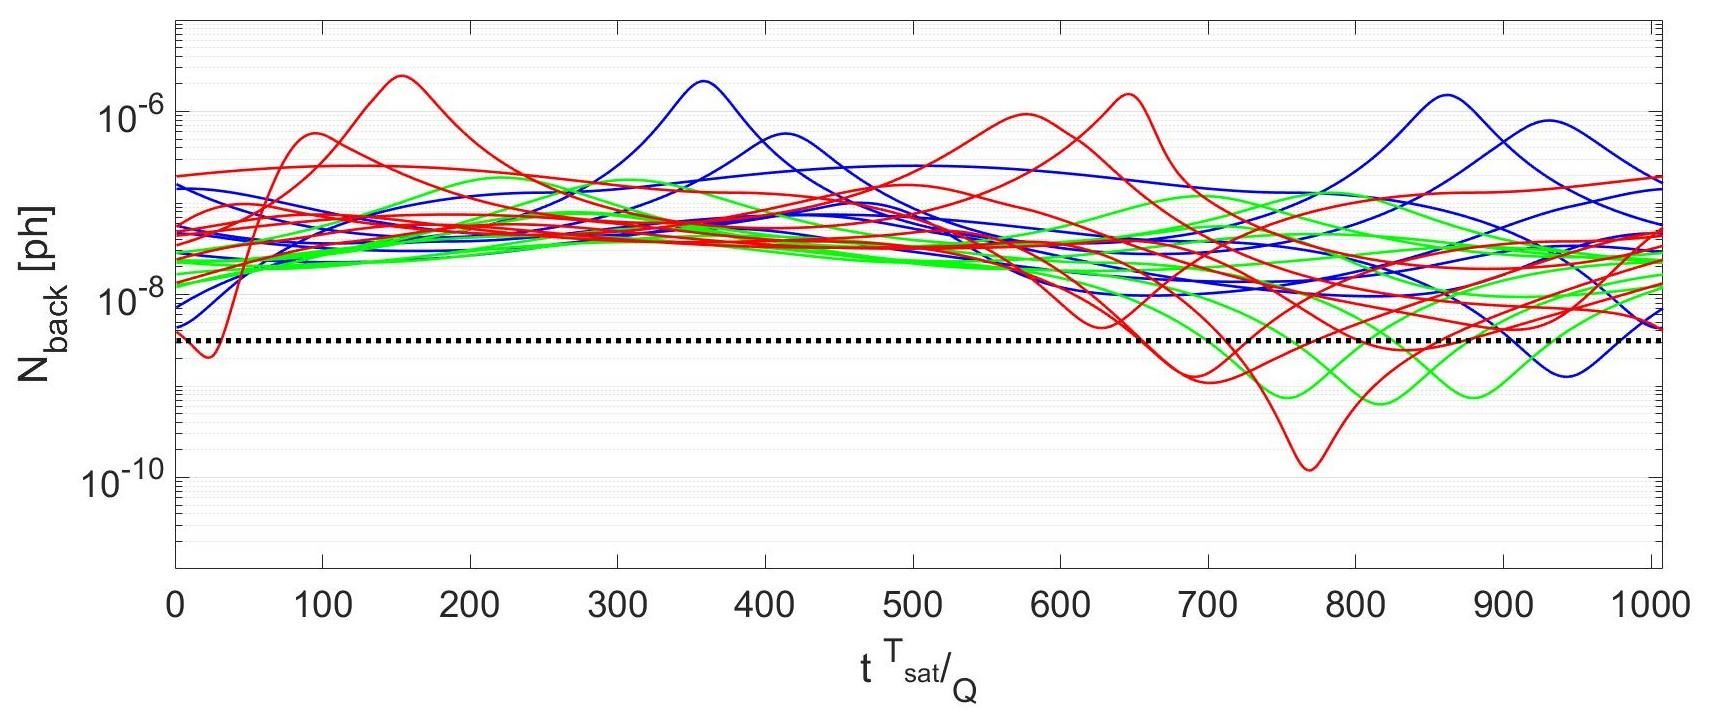
\includegraphics[width=\linewidth]{simSphere}
			\caption{Result with the spherical model}
			\label{fig:simSphere}
		\end{subfigure}
		\begin{subfigure}[b]{\linewidth}
			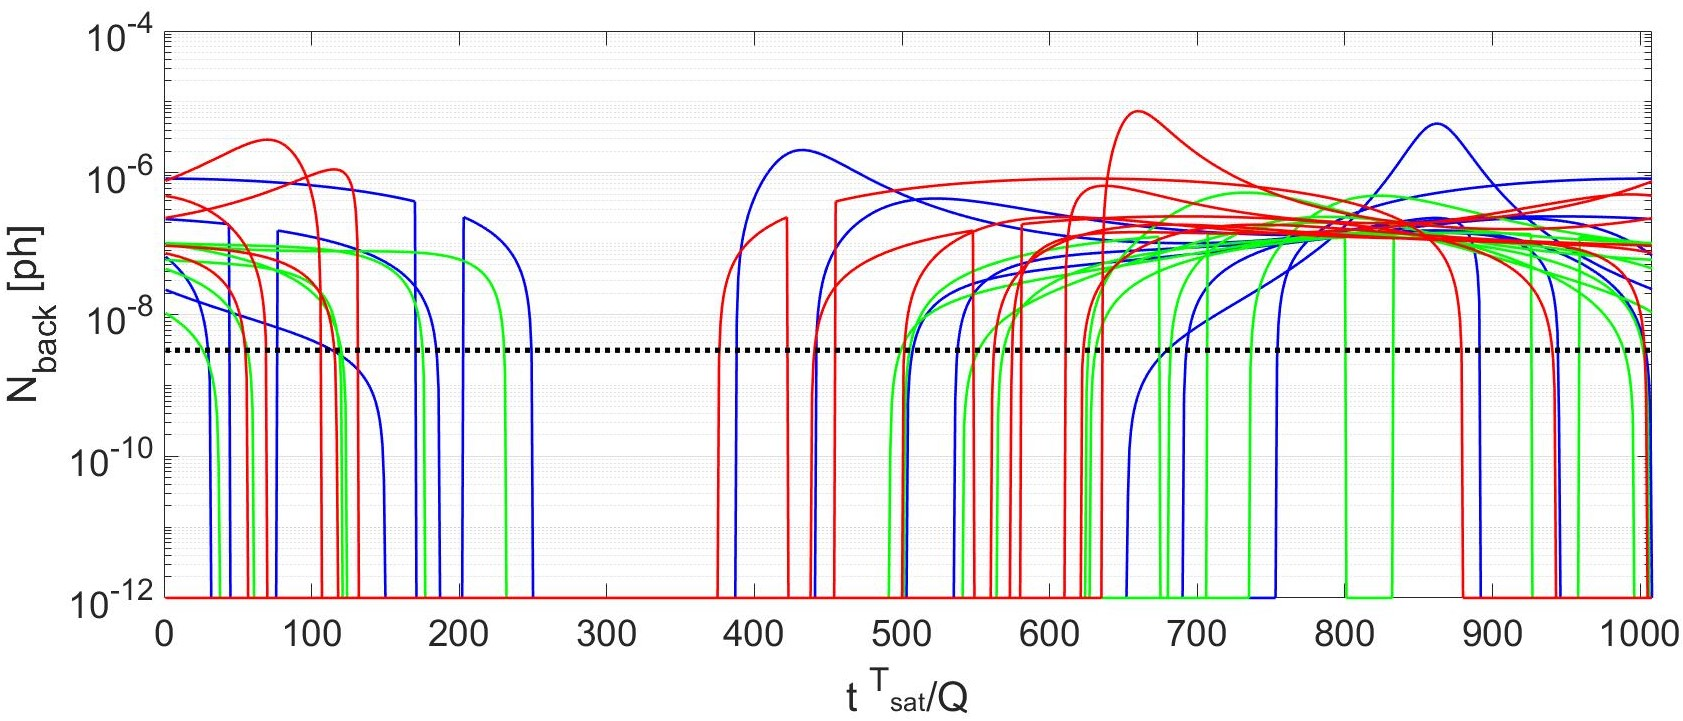
\includegraphics[width=\linewidth]{simParal}
			\caption{Result with the parallelepiped model}
			\label{fig:simParal}
		\end{subfigure}
		\caption{$N_{back}$ obtained from the simulation considering both the transmitter shapes}\label{fig:simShape}
	\end{figure}
	\section{Calculation of secret bits obtainable from each link}
	[...]
	\section{QKD network}
	[...]
	\section{Conclusions}
	[...]
	\bibliographystyle{plain}
	\bibliography{references}
	
\end{document}
